\chapter {Planning}

\section {Chemical Ideas}

	\subsection{Rate of Reactions}




	\subsection{pH}

The pH scale is composed of two extremes that describes a chemical property about the substance being tested, these extremes are called acids and bases. Mixing acids and bases together will induce a neutralisation reaction which can cancel out their extreme effects. A substance which is neither acidic nor basic is called a neutral substance. The pH scale ranges from 0 to 14, with 0 being as acidic as possible and 14 being as basic as possible. Neutral has a corresponding pH of 7 and therefore anything below 7 is acidic and anything above 7 is basic. The pH scale is illistrated below.


\begin{figure}[H]
    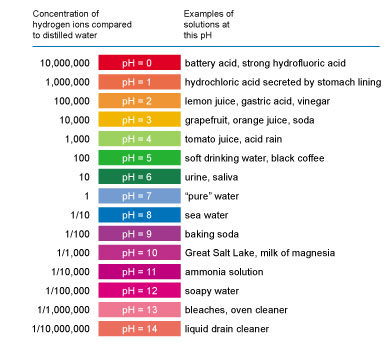
\includegraphics[width=\textwidth]{./Planning/Images/pHScale.jpg}
    \caption{The pH scale} \label{fig:pH Scale}
\end{figure}

The pH scale is a man made scale which is used to measure the concentration of hydrogen ions, each concentration is given a corresponding place on the scale (pH). pH is mathematically defined as the negative logarithm of the hydrogen ion concentration. As a result of this we can determine that the pH scale is logarithmic, therefore each value above/below the neutral value (7) is ten times more basic/acidic respectively. For example pH 6 is ten times as acidic as pH 7  and pH 5 is one hundred times as acidic than pH 7.

\begin{itemize}
\item pH = - log [H\^+]
\end{itemize}

There are many indicators used to find out the pH of substances.



	\subsection{Acids}



	\subsection{Catalysts}




	\subsection{Factors that affect Rate of Reaction}



	\subsection{Enthalpy Level Diagrams}	



	\subsection{Methods of Finding Rates}



		\subsubsection{Justification of Chosen Method}



	\subsection{How the Rate of Reaction is Determined Experimentally}



	\subsection{Rate Equations}



	\subsection{Orders of Reactions}



	\subsection{Transition Metal Catalysts}



	\subsection{D-Orbitals}



	\subsection{Complexes and their Properties}


\section{Inventory}

	\subsection{Equipment List}
\begin{itemize}
\item 250 cm3 conical flask.
\item Bung fitted to a glass tube.
\item Burette.
\end{itemize}

	\subsection{Chemical List}
\begin{itemize}
\item Distilled Water.
\item 0.20 moldm-3 Copper Sulfate (aq).
\item 1.0 moldm-3 Sulfuric Acid (aq).
\item Granulated Zinc (s).
\item Mixture of Different Catalysts.
\end{itemize}



\section{Methods}

\textbf{Setting Up}

\begin{enumerate}
\item Fill the Burette with distilled water.
\item Fit the bung (fitted with glass tube) into the conical flask.
\item Fit the inverted Burette to the end of the glass tube.
\end{enumerate}

\textbf{Carrying out the Experiment}

\begin{enumerate}
\item Remove the bung from the conical flask and pour 30 cm3 of distilled water and 10 cm3 of sulfuric acid into the conical flask.
\item Weigh out 1.0 g of granulated zinc.
\item Add the measured 1.0 g of granulated zinc to the conical flask.
\item Place the bung back in the conical flask.
\item Record the volume of hydrogen produced in cm3 every 30 seconds for 5 minutes from the burette markings to 1 decimal place.
\item Repeat the experiment but use 30cm3 of copper sulfate instead of distilled water.
\end{enumerate} 

\textbf{Interpreting the Data}

\begin{enumerate}
\item Plot a graph of the volume of hydrogen against time.
\item From the graph draw a tangent to the line at the initial point.
\item Calculate the gradient of the tangent by using the equation: 
\item The gradient is equal to the rate of reaction.
\end{enumerate}



	\subsection{Justification of Chosen Method}


\section{Risk Assessment}